\documentclass[%
pdf,
%nocolorBG,
colorBG,
slideColor,
%slideBW,
%draft,
%frames
%azure
%contemporain
%nuancegris
%troispoints
%lignesbleues
%darkblue
%alienglow
%autumn
]{prosper}
\usepackage{pifont, amsmath, multicol}
%\usepackage{floatflt, wrapfig,subfigure}
%\usepackage{wrapfig}
\usepackage{floatflt}
\usepackage[dvips]{color}
\usepackage{epsfig}
\usepackage{pifont}
%\usepackage[francais]{babel}
\usepackage[T1]{fontenc}
\usepackage[latin1]{inputenc}
%\def«{\og\ignorespaces}%
%\def»{{\fg}}%
\newcommand{\spacer}{\rule[-3mm]{0mm}{8mm}}

\newcommand{\RR}{\ensuremath{\mathbb{R}}}
\newcommand{\NN}{\ensuremath{\mathbb{N}}}
\newcommand{\QQ}{\ensuremath{\mathbb{Q}}}
\newcommand{\CC}{\ensuremath{\mathbb{C}}}
\newcommand{\ZZ}{\ensuremath{\mathbb{Z}}}
\newcommand{\TT}{\ensuremath{\mathbb{T}}}

\def\QuotS#1#2{\leavevmode\kern-.0em\raise.2ex\hbox{$#1$}\kern-.1em/\kern-.1em\lower.25ex\hbox{$#2$}}


\title{\Huge \textcolor{blue}{Polycycles and}\\[3mm]
\textcolor{blue}{face-regular two-maps}}

\author{
\textcolor{red}{\Large Mathieu Dutour,}\\[2mm]
\textcolor{red}{\Large Michel Deza}\\[2mm]
\textcolor{red}{\Large and Mikhail Shtogrin}\\
}
\author{
\textcolor{red}{\Large Mathieu Dutour}\\[2mm]
\textcolor{red}{\large ENS/CNRS, Paris and Hebrew University, Jerusalem}\\[2mm]
\textcolor{red}{\Large Michel Deza}\\[2mm]
\textcolor{red}{\large ENS/CNRS, Paris and ISM, Tokyo}\\[2mm]
\textcolor{red}{\Large and Mikhail Shtogrin}\\[2mm]
\textcolor{red}{\large Steklov Institute, Moscow}
}


\slideCaption{}

\date{}



\begin{document}
\maketitle

















\begin{slide}{}
\begin{center}
{\Huge 
\begin{tabular*}{9cm}{c}
\\[-0.5cm]
\textcolor{blue}{I. }\textcolor{red}{Strictly}\\
\textcolor{red}{face-regular two-maps}
\end{tabular*}
}
\end{center}
\end{slide}




\begin{slide}{Definition}
\vspace{-3mm}
A \textcolor{red}{strictly face-regular two-map} is 
\begin{itemize}
\item a $3$-connected!! $3$-valent map (on sphere or torus), whose faces 
have size $p$ 
or $q$ (\textcolor{red}{$(p,q)$-sphere} or \textcolor{red}{$(p,q)$-torus})
\item \textcolor{red}{$pR_i$} holds: any $p$-gonal face is!! 
adjacent to $i$ $p$-gonal faces
\item \textcolor{red}{$qR_j$} holds: any $q$-gonal face is!!
adjacent to $j$ $q$-gonal faces
\end{itemize}

\begin{center}
\begin{minipage}{4.7cm}
\centering
\resizebox{3.8cm}{!}{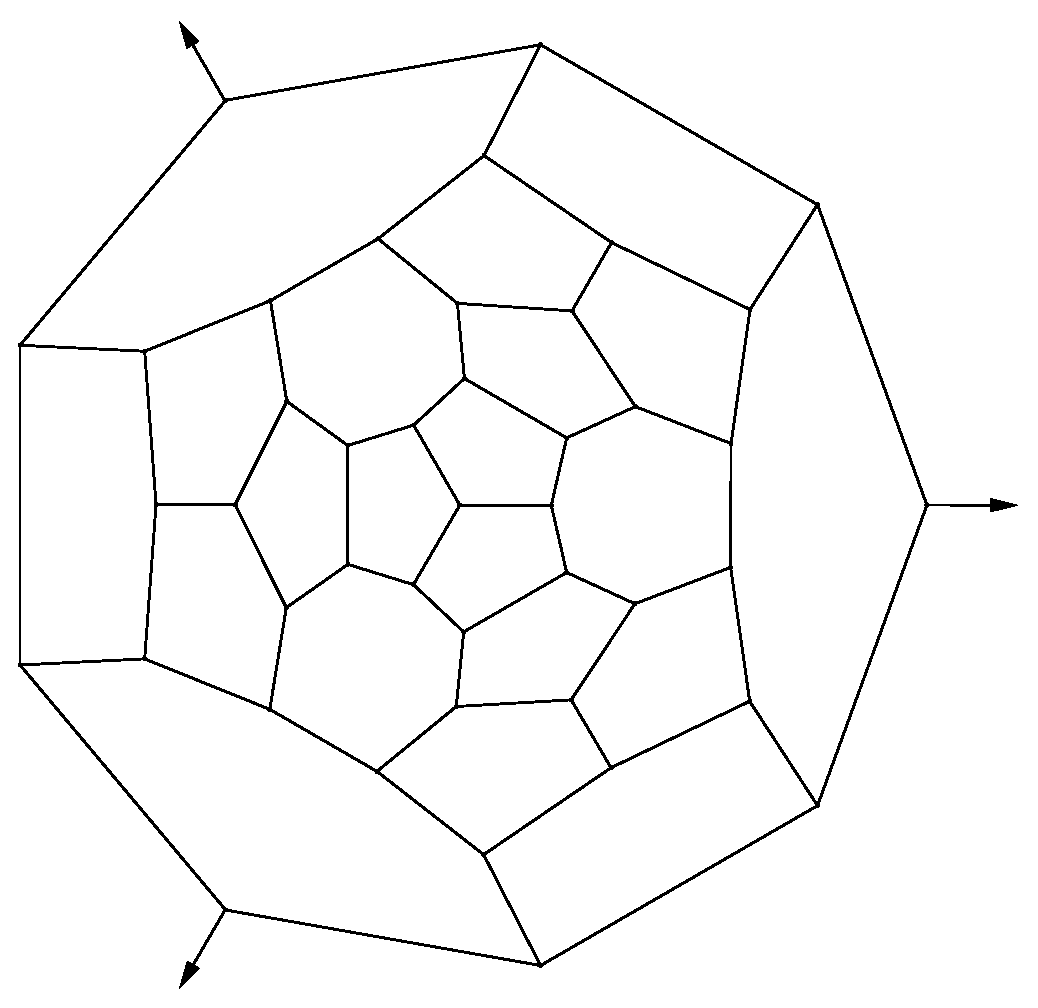
\includegraphics{FaceRegular/Graph57_5R3_7R1sec.eps}}\par
$(5,7)$-sphere $5R_3$, $7R_1$
\end{minipage}
\begin{minipage}{4.7cm}
\centering
\resizebox{3.8cm}{!}{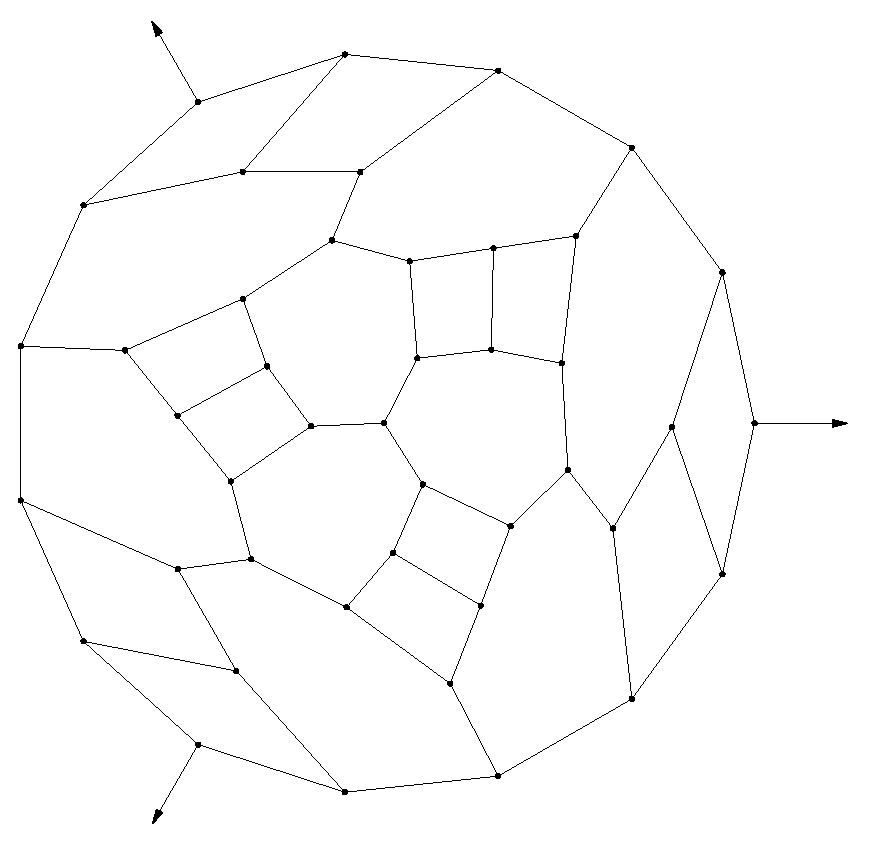
\includegraphics{FaceRegular/FaceReg_4R1_7R4sec.eps}}\par
$(4,7)$-sphere $4R_1$, $7R_4$
\end{minipage}

\end{center}
\end{slide}







\begin{slide}{Euler formula}
\begin{itemize}
\item If $e_{p-q}$ denote the number of edges 
separating $p$- and $q$-gon, then one has:
\begin{equation*}
e_{p-q}=(p-i)f_p=(q-j)f_q
\end{equation*}
\item Euler formula $V-E+F=2-2g$ with $g$ being the genus,!! 
can be rewritten as
\begin{equation*}
(6-p)f_p+(6-q)f_q=6(2-2g)
\end{equation*}
\item This implies
\begin{equation*}
e_{p-q}\textcolor{red}{\{\frac{6-p}{p-i}+\frac{6-q}{q-j}\} }=e_{p-q}\textcolor{red}{\alpha(p,q,i,j)}=12(1-g)
\end{equation*}
\end{itemize}


\end{slide}








\begin{slide}{A classification}
!!%Three cases are possible:
\begin{itemize}
\item If $\alpha(p,q,i,j)>0$, then $g=0$, the map exists only on sphere and the number of vertices depends only on $\alpha(p,q,i,j)$.
\item If $\alpha(p,q,i,j)=0$, then $g=1$, the map exists only on torus.
\item If $\alpha(p,q,i,j)<0$, then $g>1$, the map exists only on surfaces of higher genus and the number of vertices is determined by the genus and $\alpha(p,q,i,j)$.
\end{itemize}
Detailed classification:
\begin{itemize}
\item \textcolor{red}{On sphere}: $55$ sporadic examples + two infinite 
series: $Prism_q$ ($q \ge 3, q \neq 4$)!! and $Barrel_q$ ($q \ge 3, q 
\neq 5$)!!
\item \textcolor{red}{On torus}: $7$ sporadic examples + $16$ 
infinities.!! 
!!%infinity of possibilities.
!!excusion of above and first lines is needed, since now you not fit!!
\end{itemize}


\end{slide}




\begin{slide}{Sporadic tori}

\begin{center}
\begin{minipage}{3.75cm}
\centering
\resizebox{3.3cm}{!}{\includegraphics[bb=150 266 476 540, clip]{FaceRegular/UniqueTorus312_12R6.eps}}\par
$(6,12)$-torus $3R_0$, $12R_6$
\end{minipage}
\begin{minipage}{3.75cm}
\centering
\resizebox{3.3cm}{!}{\includegraphics[bb=150 266 476 540, clip]{FaceRegular/UniqueTorus48_8R4.eps}}\par
$(4,8)$-torus $4R_0$, $8R_4$
\end{minipage}
\begin{minipage}{3.75cm}
\centering
\resizebox{3.3cm}{!}{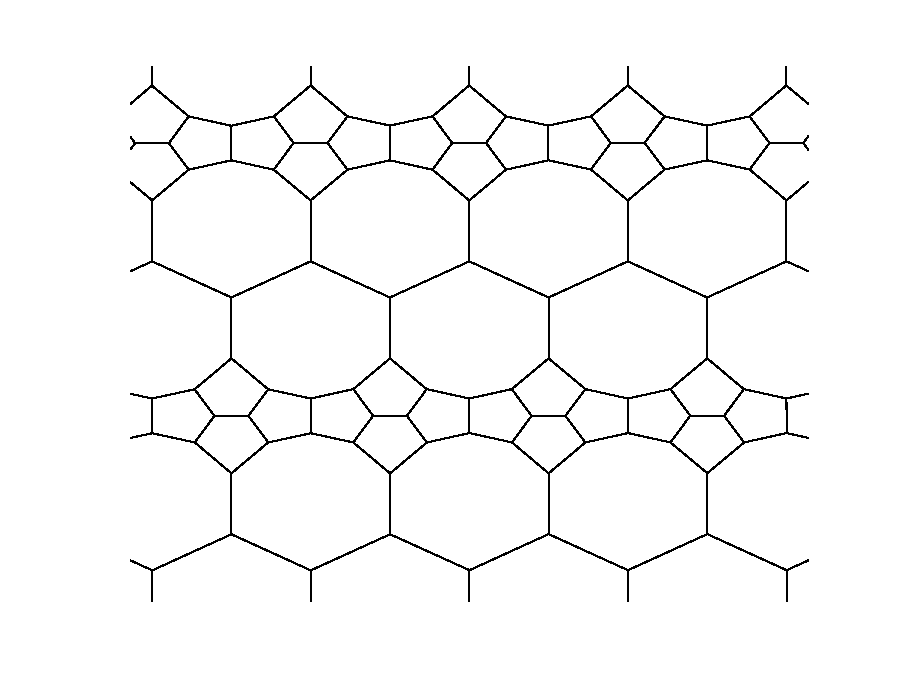
\includegraphics[bb=150 266 476 540, clip]{FaceRegular/UniqueStrictly8R4_5R3.eps}}\par
$(5,8)$-torus $5R_3$, $8R_4$
\end{minipage}
\begin{minipage}{3.75cm}
\centering
\resizebox{3.3cm}{!}{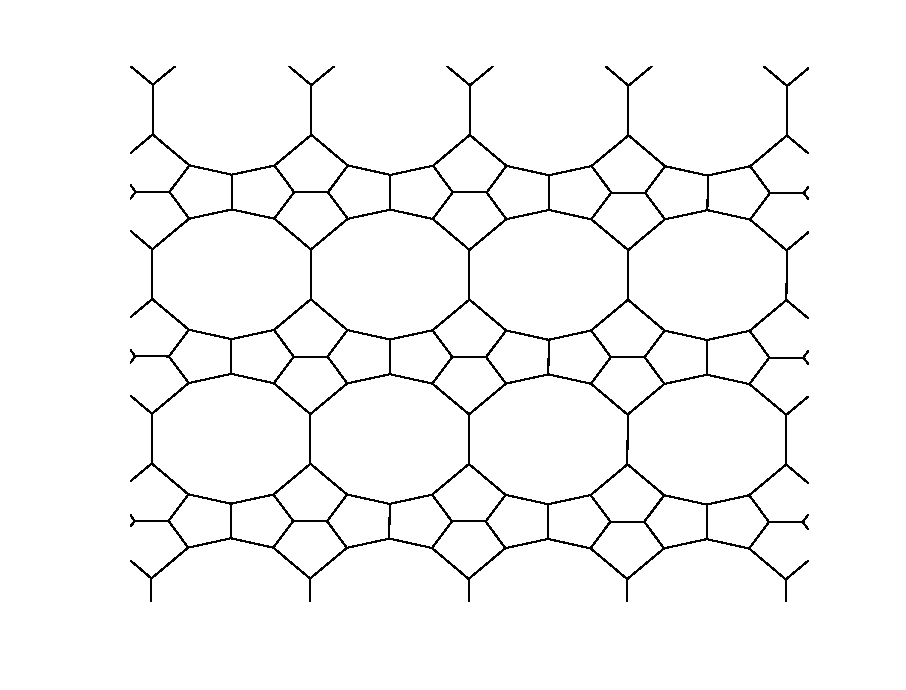
\includegraphics[bb=150 266 476 540, clip]{FaceRegular/UniqueStrictly10R2_5R3.eps}}\par
$(5,10)$-torus $5R_3$, $10R_2$
\end{minipage}
\begin{minipage}{3.75cm}
\centering
\resizebox{3.3cm}{!}{\includegraphics[bb=150 266 476 540, clip]{FaceRegular/UniqueStrictly11R1_5R3.eps}}\par
$(5,11)$-torus $5R_3$, $11R_1$
\end{minipage}
\begin{minipage}{3.75cm}
\centering
\resizebox{3.3cm}{!}{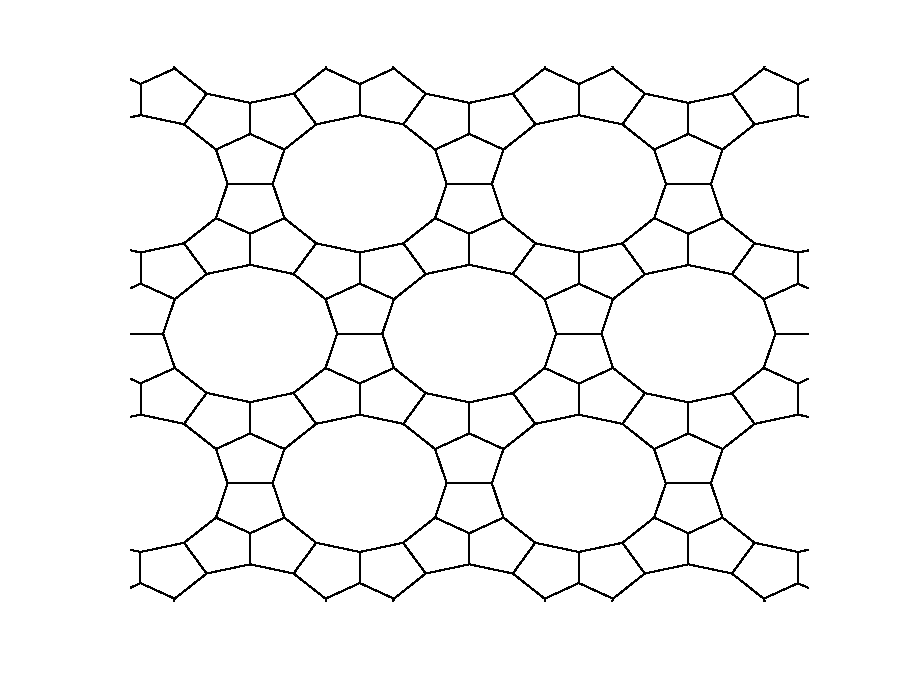
\includegraphics[bb=150 266 476 540, clip]{FaceRegular/UniqueStrictly12R0_5R3.eps}}\par
$(5,12)$-torus $5R_3$, $12R_0$
\end{minipage}
!!now you not fit in page; a solution is to do text under each picture 
by small, then you will save 2 needed lines. Other thing: pity that you 
could not put the last, 7th sporadic torus; perhaps?? diminish all and put 
it in also?!! 
\end{center}


\end{slide}


\begin{slide}{$(3,q)$-tori $3R_0$, $qR_6$}
\begin{itemize}
\item They are obtained by truncating 
!!%a 
the!! $3$-valent tesseletion of the torus by $6$-gons 
!!%and 
on!! the!! vertices!! from!! a set $S_h$,!! 
!!%of vertices,
such that every face is incident to exactly!! $h$ vertices in $S_h$. 
\item There is an infinity of possibilities except for $h=6$.
\begin{center}
\begin{minipage}{3.5cm}
\centering
\resizebox{3.3cm}{!}{\includegraphics[bb=150 266 476 540, clip]{FaceRegular/Torus37_3R0_7R6_1.eps}}\par
a $(3,7)$-torus $3R_0$, $7R_6$
\end{minipage}
\begin{minipage}{3.5cm}
\centering
\resizebox{3.3cm}{!}{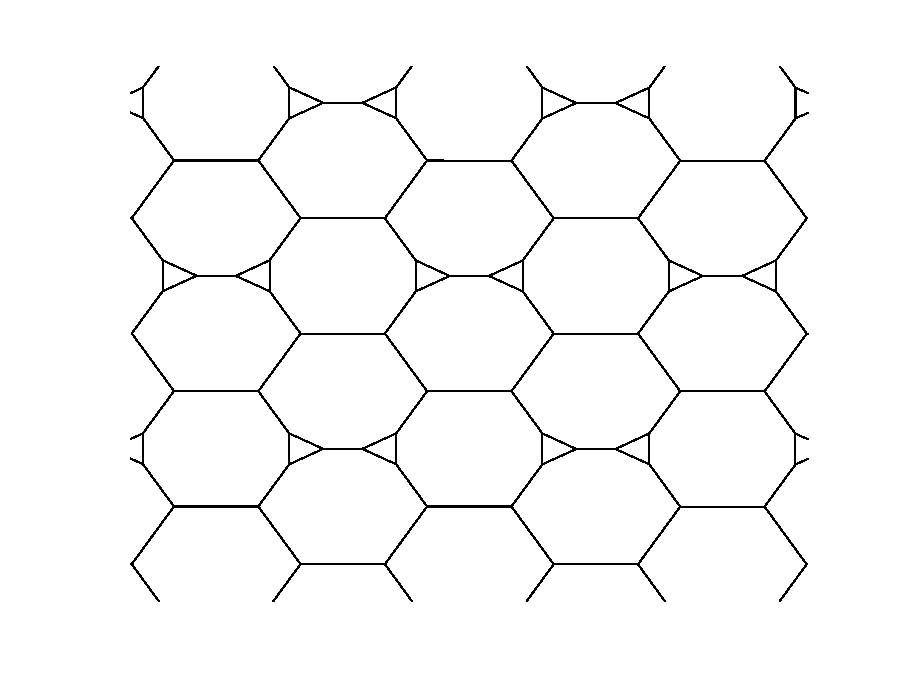
\includegraphics[bb=150 266 476 540, clip]{FaceRegular/Torus38_3R0_8R6_1.eps}}\par
a $(3,8)$-torus $3R_0$, $8R_6$
\end{minipage}
\begin{minipage}{3.5cm}
\centering
\resizebox{3.3cm}{!}{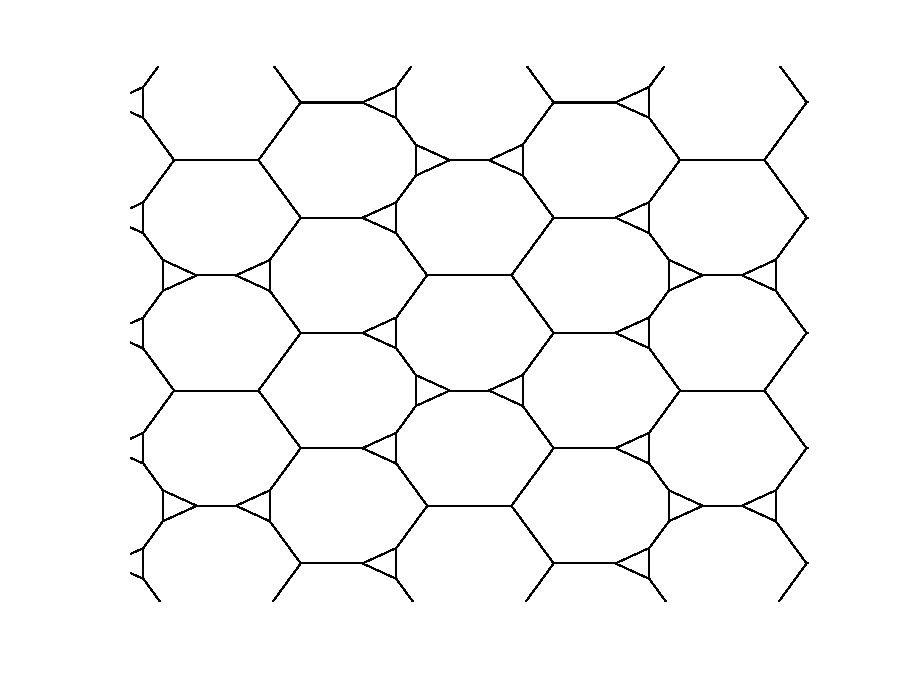
\includegraphics[bb=150 266 476 540, clip]{FaceRegular/Torus39_3R0_9R6_10.eps}}\par
a $(3,9)$-torus $3R_0$, $9R_6$
\end{minipage}
!!again, do text under tori smaller and save a line!!
\end{center}
\item $(4,q)$-tori $4R_2$, $qR_6$ are obtained by 
$4$-truncation
!!this need explanation (about 1,5 lines; you will have this place if 
folow my above advice)!!


\end{itemize}
\end{slide}




\begin{slide}{$(4,10)$-tori $4R_1$, $10R_4$}
\begin{itemize}
\item Take the 
!!%two 
symbols
\begin{center}
\begin{minipage}{5.3cm}
\centering
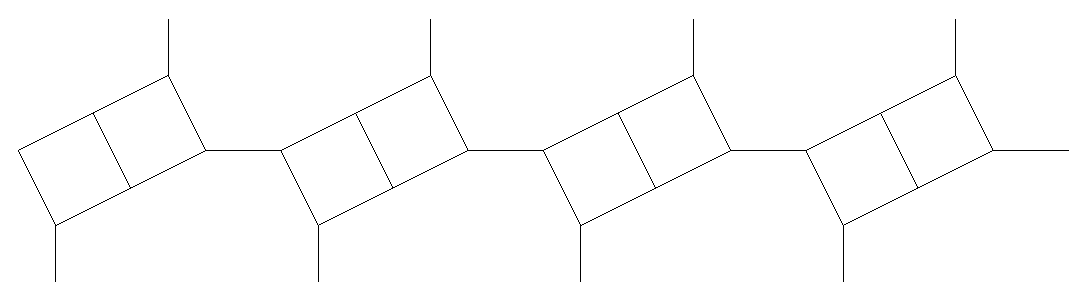
\epsfig{height=12mm, file=RedCont16_1.eps}\par
$u$
\end{minipage}
\begin{minipage}{5.3cm}
\centering
\epsfig{height=12mm, file=RedCont16_2.eps}\par
$v$
\end{minipage}
\end{center}
\item The torus correspond to words of the form $(\alpha_0\dots\alpha_n)^{\infty}$ with $\alpha_i$ being equal to $u$ or $v$.
\begin{center}
\begin{minipage}{5.2cm}
\centering
\resizebox{4.0cm}{!}{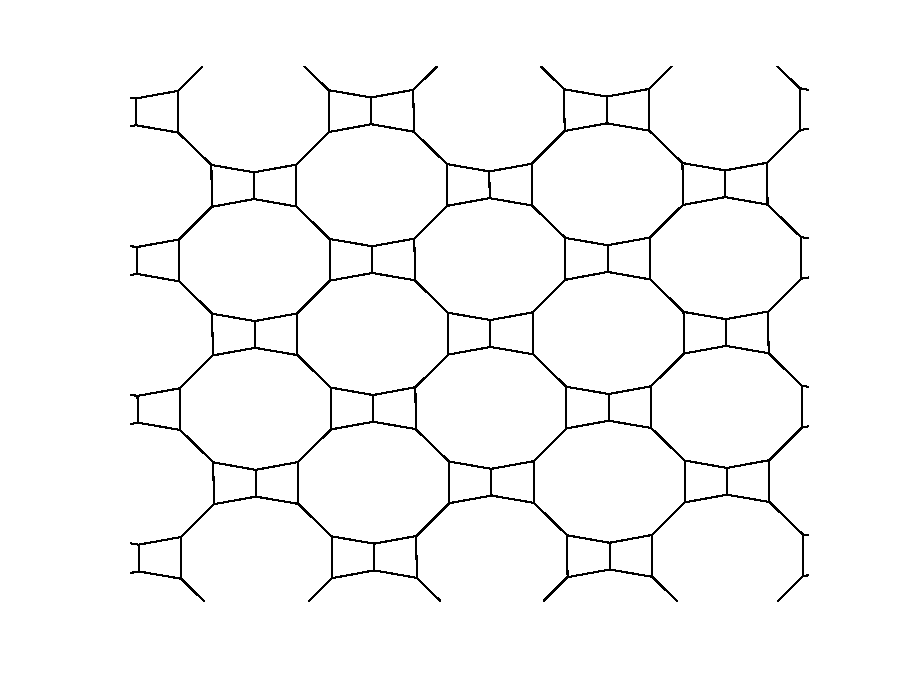
\includegraphics[bb=150 266 476 540, clip]{FaceRegular/Torus410_4R1_10R4_14.eps}}\par
$(u)^{\infty}$
\end{minipage}
\begin{minipage}{5.2cm}
\centering
\resizebox{4.0cm}{!}{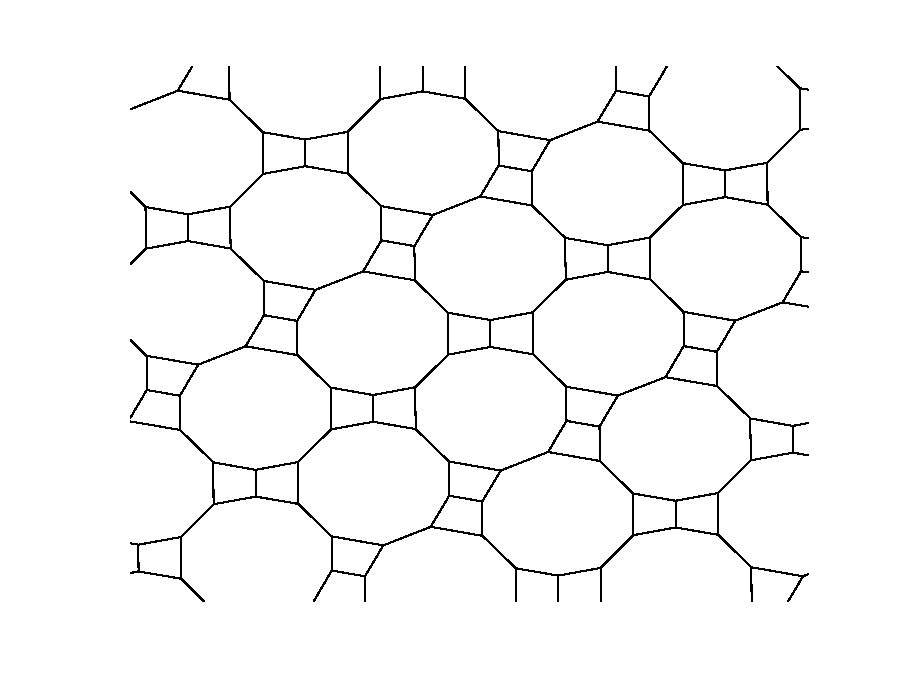
\includegraphics[bb=150 266 476 540, clip]{FaceRegular/Torus410_4R1_10R4_16.eps}}\par
$(uv)^{\infty}$
\end{minipage}
!!do above tori smaller: now you not fit!!
\end{center}

\end{itemize}
\end{slide}


\begin{slide}{$(5,7)$-tori $5R_1$, $7R_3$}
\begin{itemize}
\item Take the symbols
\begin{center}
\begin{minipage}{5.3cm}
\centering

\epsfig{height=13mm, file=RedCont17_1.eps}\par
$u$
\end{minipage}
\begin{minipage}{5.3cm}
\centering
\epsfig{height=13mm, file=RedCont17_2.eps}\par
!!%and 
$v$
\end{minipage}
\end{center}
\item The torus correspond to words of the form 
$(\alpha_0\dots\alpha_n)^{\infty}$ 
with $\alpha_i$ being equal to $u$ or $v$.
!!now you not fit; so, either delete above line (since alpha was 
explained before) or do tori below smaller!!
\begin{center}
\begin{minipage}{5.2cm}
\centering
\resizebox{4.0cm}{!}{\includegraphics[bb=150 266 476 540, clip]{FaceRegular/Torus57_5R1_1.eps}}\par
$(u)^{\infty}$
\end{minipage}
\begin{minipage}{5.2cm}
\centering
\resizebox{4.0cm}{!}{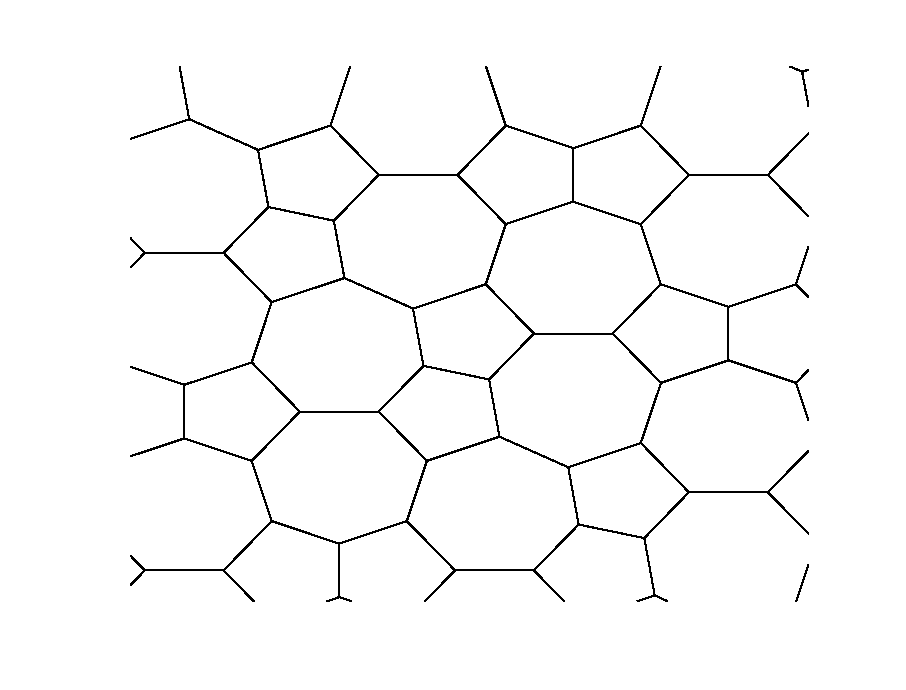
\includegraphics[bb=150 266 476 540, clip]{FaceRegular/Torus57_5R1_2.eps}}\par
$(uv)^{\infty}$
\end{minipage}
\end{center}

\end{itemize}
\end{slide}










\begin{slide}{$(5,7)$-tori!! $5R_2$, $7R_4$}
\begin{itemize}
\item $5$-gons 
!!%in 
forming!! an!! infinite line, \textcolor{red}{one possibility}
\begin{center}
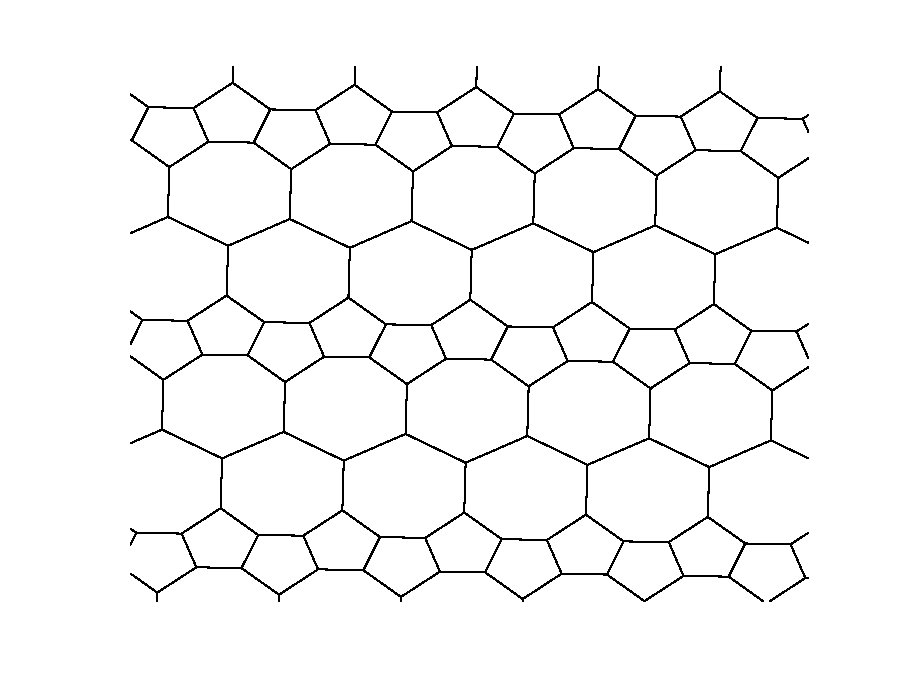
\epsfig{height=30mm, file=FaceRegular/Unique57_LinesOf2.eps}\par
\end{center}
\item Take the symbols
\begin{center}
\begin{minipage}{5.2cm}
\centering
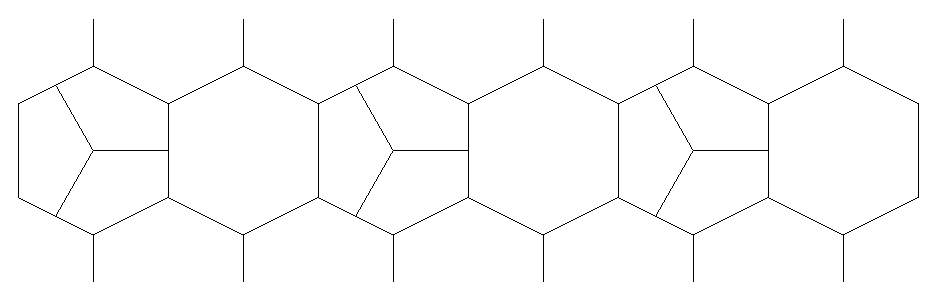
\epsfig{height=13mm, file=RedCont18_1.eps}\par
$u$
\end{minipage}
\begin{minipage}{5.2cm}
\centering
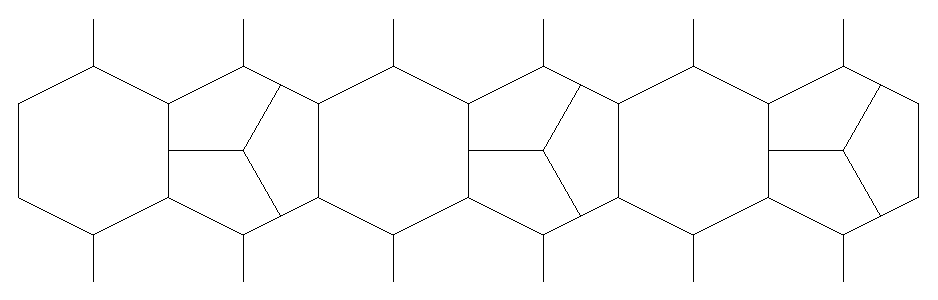
\epsfig{height=13mm, file=RedCont18_2.eps}\par
!!%and 
$v$
\end{minipage}
\end{center}
\item Other tori correspond to words of the form 
$(\alpha_0\dots\alpha_n)^{\infty}$ 
with $\alpha_i$ being equal to $u$ or $v$.
!!delete above line, because now you not fit and because alpha was already
explained!!
%\begin{center}
%\begin{minipage}{5.2cm}
%\centering
%\resizebox{5.0cm}{!}{\includegraphics[bb=150 266 476 540, clip]{FaceRegular/Torus57_5R2_7R4_u.eps}}\par
%$(u)^{\infty}$
%\end{minipage}
%\begin{minipage}{5.2cm}
%\centering
%\resizebox{5.0cm}{!}{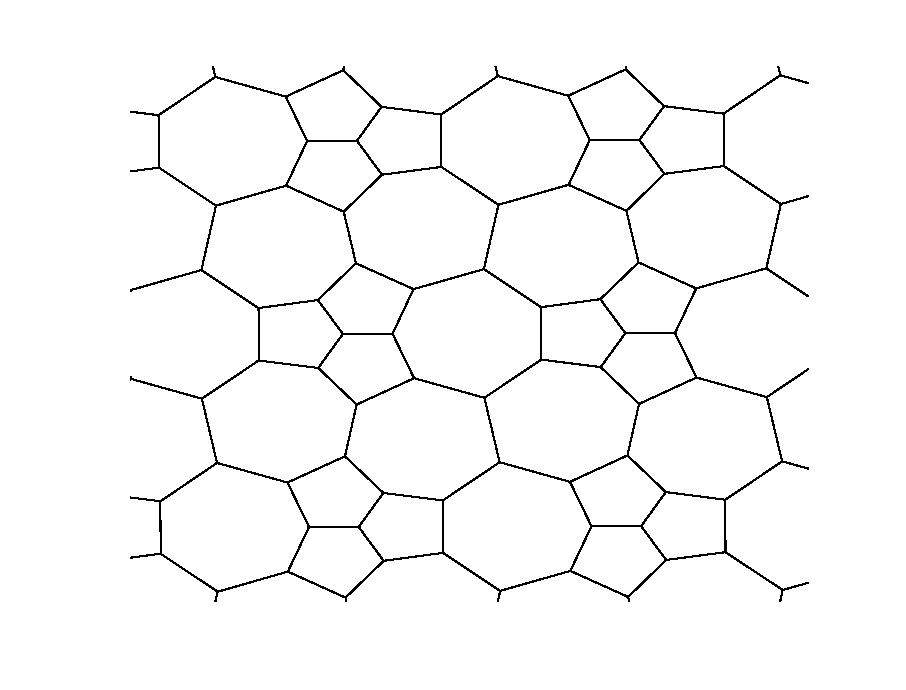
\includegraphics[bb=150 266 476 540, clip]{FaceRegular/Torus57_5R2_7R4_uv.eps}}\par
%$(uv)^{\infty}$
%\end{minipage}
%\end{center}


\end{itemize}
\end{slide}




\begin{slide}{$(5,8)$-tori $5R_2$, $8R_2$}
\begin{itemize}
\item $5$-gons and $8$-gons are organized in infinite lines.
\item 
!!%Two 
Only!! two!! configurations for $5$-gons locally:
\begin{center}
\begin{minipage}{5.2cm}
\centering
\epsfig{height=13mm, file=3_5_polycycle_1.eps}\par
$u$
\end{minipage}
\begin{minipage}{5.2cm}
\centering
\epsfig{height=13mm, file=3_5_polycycle_2.eps}\par
!!%and 
$v$
\end{minipage}
\end{center}
\item Words of the form $(\alpha_0\dots\alpha_n)^{\infty}$ with $\alpha_i$ being equal to $u$ or $v$ and $uuu$, $vvv$ being forbidden.



\end{itemize}
\end{slide}



\overlays{2}{
\begin{slide}{$(4,8)$-tori $4R_1$, $8R_5$}
\fromSlide{1}{
\begin{itemize}
\item They are in one-to-one correspondance with 
\textcolor{red}{perfect matchings!!} of the!! $6$-regular triangulation!! 
of the 
torus,!! such that every vertex is contained in 
a triangle whose opposite edges!! 
!!strange line above: any two edges of a triangle are opposite!!
belong to the perfect matching.
\end{itemize}
}%
\onlySlide*{1}{
\begin{center}
\begin{minipage}{8.2cm}
\centering
\resizebox{7.0cm}{!}{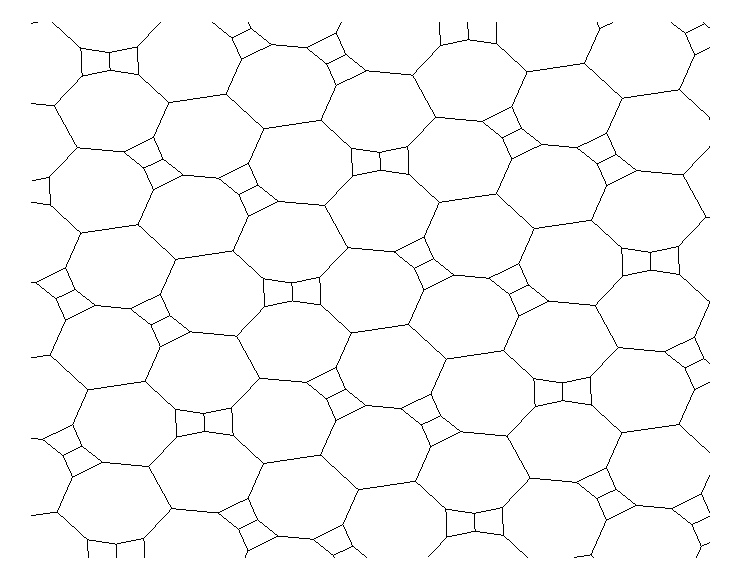
\includegraphics{Torus48_4R1_8R5_5_BS.eps}}\par
\end{minipage}
\end{center}
}%
\onlySlide*{2}{
\begin{center}
\begin{minipage}{8.2cm}
\centering
\resizebox{7.0cm}{!}{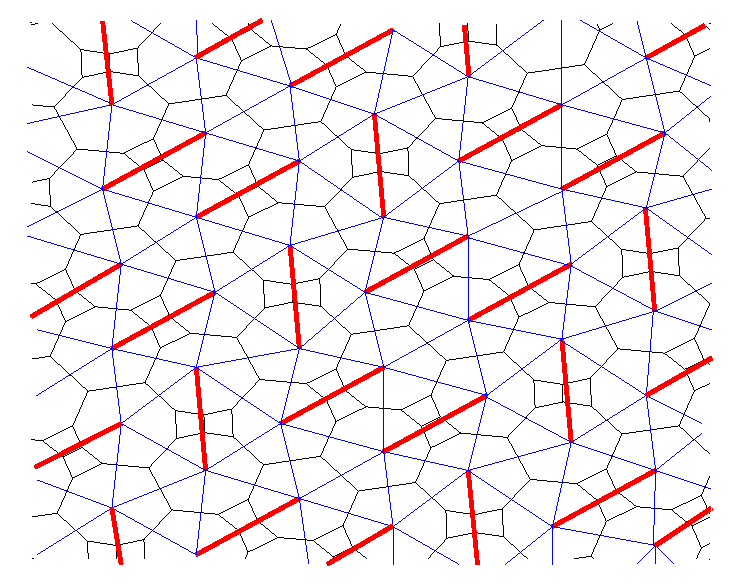
\includegraphics{Torus48_4R1_8R5_5_PM.eps}}\par
\end{minipage}
\end{center}
}%

\end{slide}
}





\begin{slide}{$(4,7)$-tori $4R_0$, $7R_5$}
\begin{itemize}
\item This case is not classified.
\item The following example shows the difficulty of 
!!%a 
the!! classification.
!!above line needs clarification and you have small space: 1-2 lines, 
for it!!
\begin{center}
\begin{minipage}{5.2cm}
\centering
\resizebox{5.0cm}{!}{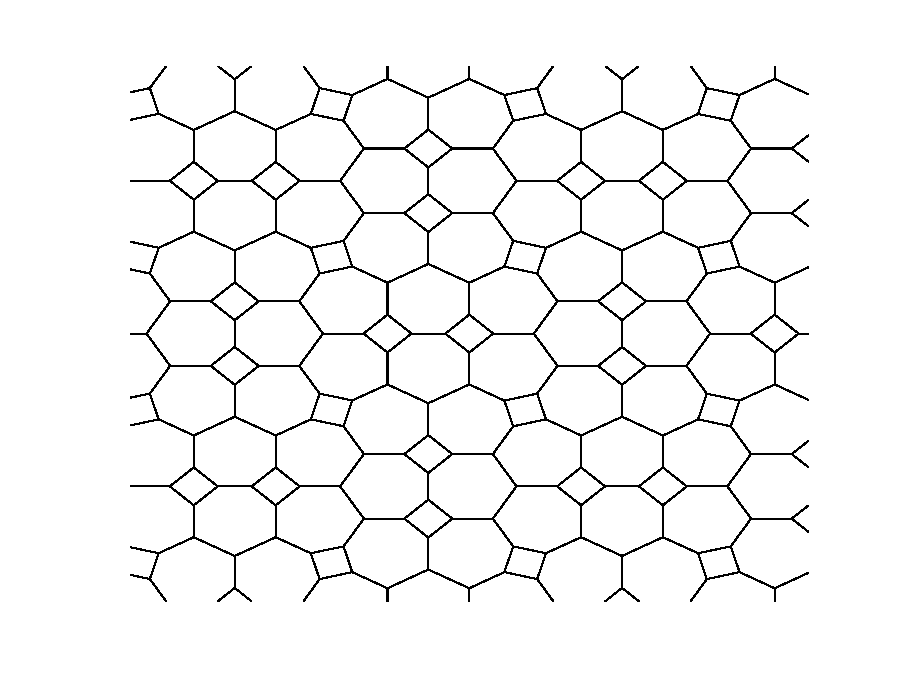
\includegraphics[bb=150 266 476 540, clip]{FaceRegular/Torus47_4R0_7R5_22.eps}}\par
\end{minipage}
\end{center}

\end{itemize}
\end{slide}




\begin{slide}{}
\begin{center}
{\Huge 
\begin{tabular*}{7cm}{c}
\\[-0.5cm]
\textcolor{blue}{II. }\textcolor{red}{$(p,3)$-polycycles}
\end{tabular*}
}
\end{center}
\end{slide}



%$G$ of girth $p$ and maximal vertex-degree $s$, which admits
%a realization on the plane, such that:

\begin{slide}{$(p,3)$-polycycles}
a \textcolor{red}{generalized $(p,3)!!$-polycycle} is a 
$2$-connected plane 
graph with faces partitionned in two families $F_1$
!!%,
and!! $F_2$, so that:
\begin{itemize}
\item all elements of $F_1$ (\textcolor{red}{proper faces}) are
(combinatorial)!! $p$-gons
!!%) 
and:!!
\item all elements of $F_2$ (\textcolor{red}{holes}, the exterior face
is amongst them) are pair-wisely disjoint;
\item all verices have valency $3$ or $2$ and any $2$-valent vertex lies on a 
boundary of a hole.
!!ADD, perhaps: A $(5,3)$-polycycle: if the exterior face is unique 
hole.!!
\end{itemize}

\begin{center}
\epsfig{file=Boundary/3_5_polycycle.eps, width=4cm}
\end{center}

\end{slide}







\begin{slide}{$(3,3)$ and $(4,3)$-polycycles}
{\it\scriptsize

%{\bf Theorem}

(i) \textcolor{red}{Any $(3,3)$-polycycle} is one of the following $3$ cases:
\begin{center}
\epsfig{figure=Boundary/Possible3gonalPatchNOB.eps,width=6cm}
\end{center}

(ii) \textcolor{red}{Any $(4,3)$-polycycle} belongs to the following $3$ cases:
\begin{center}
\epsfig{figure=Discrete4gonal_SEC.eps,width=6cm}
\end{center}
\hspace{1cm}or belong to the following infinite family of $(4,3)$-polycycles:
\begin{center}
\epsfig{figure=Boundary/InfiniteSequenceNOB.eps,width=8cm}
\end{center}

}
This classification is very useful for classifying $(4,q)$-maps.

\end{slide}





\overlays{7}{
\begin{slide}{Polycycle decompositions}
\onlySlide*{1}{
!!%We can generalize a polycycle by allowing \textcolor{red}{several} 
!!%boundaries. 
An example of a generalized $(5,3)$-polycycle:
!!move,perhaps, this example above, just after definitition of gener. 
polycycle!!
\begin{center}
\resizebox{6cm}{!}{\includegraphics{PolycycleFig2.eps}}
\end{center}
}
\onlySlide*{2}{
A \textcolor{red}{frontier} is an edge going from a 
!!%boundary to a boundary.
hole!! to!! another!! hole.!!
!!Perhaps, term "bridge" will be better than "frontier", which looks as 
a "boundary".!!
 \\[1.3cm]
\begin{center}
\resizebox{6cm}{!}{\includegraphics{PolycycleFig3.eps}}
\end{center}
}
\onlySlide*{3}{
Any!!  generalized polycycle is \textcolor{red}{uniquely decomposable!!} 
along its frontiers.
\begin{center}
\resizebox{9cm}{!}{\includegraphics{PolycycleFig4.eps}}
\end{center}
}
\onlySlide*{4}{
\textcolor{red}
!!%{Thm.} 
The set of \textcolor{red}{non-decomposable} $(5,3)$-polycycles 
has been classified:
\begin{center}
\begin{minipage}{3.7cm}
\centering
\resizebox{3.0cm}{!}{\includegraphics{Polycycle/Dodecahedron.eps}}\par
\end{minipage}
\begin{minipage}{3.7cm}
\centering
\resizebox{3.0cm}{!}{\rotatebox{90}{\includegraphics{Polycycle/PolycycleA2.eps}}}\par
\end{minipage}
\begin{minipage}{3.7cm}
\centering
\resizebox{3.0cm}{!}{\includegraphics{Polycycle/Dodecahedron3vertDegTwo.ps}}\par
\end{minipage}
\begin{minipage}{3.7cm}
\centering
\resizebox{3.0cm}{!}{\includegraphics{Polycycle/PolycycleA4.eps}}\par
\end{minipage}
\begin{minipage}{3.7cm}
\centering
\resizebox{3.0cm}{!}{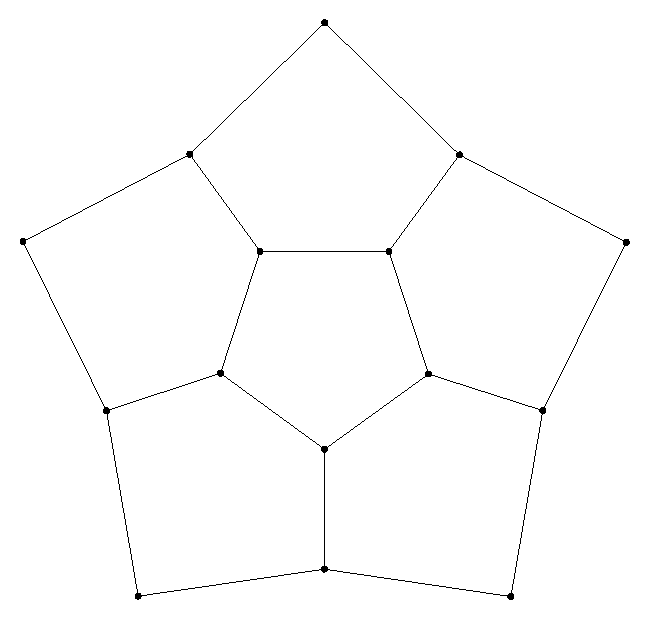
\includegraphics{Polycycle/PolycycleA5.eps}}\par
\end{minipage}
\begin{minipage}{3.7cm}
\centering
\resizebox{2.0cm}{!}{\rotatebox{180}{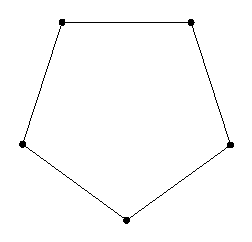
\includegraphics{Polycycle/PolycycleD.eps}}}\par
\end{minipage}
\end{center}
}
\onlySlide*{5}{
\begin{center}
\begin{minipage}{3.7cm}
\centering
\resizebox{3.0cm}{!}{\includegraphics{Polycycle/PolycycleB2.eps}}\par
\end{minipage}
\begin{minipage}{3.7cm}
\centering
\resizebox{3.0cm}{!}{\rotatebox{90}{\includegraphics{Polycycle/PolycycleB3sec.eps}}}\par
\end{minipage}
\begin{minipage}{3.7cm}
\centering
\resizebox{3.0cm}{!}{\includegraphics{Polycycle/Fundamental22polycycle3.eps}}\par
\end{minipage}
\begin{minipage}{3.7cm}
\centering
\resizebox{2.5cm}{!}{\includegraphics{Polycycle/Elementary53_C2.eps}}\par
\end{minipage}
\begin{minipage}{3.7cm}
\centering
\resizebox{3.0cm}{!}{\includegraphics{Polycycle/Fundamental22polycycle2.eps}}\par
\end{minipage}
\begin{minipage}{3.7cm}
\centering
\epsfig{height=14mm, file=Polycycle/Fundamental22polycycle1.eps}\par
\end{minipage}
\end{center}
}
\onlySlide*{6}{
The \textcolor{red}{infinite series} of non-decomposable 
$(5,3)$-polycycles!! $E_n, n \ge 1$:!!
\\[1cm]
\begin{center}
\begin{minipage}{4.7cm}
\centering
!!put here the $E_1$, which is now last on previous slide; on liberated 
place put the 5-gon, which is now the last on pre-previous slide.
Less important but useful will be; a) to move B_3 (now second on 
previous slide) to 5th place of pre-previous slide, puching its occupant 
on already liberated 6th place.!! 
\epsfig{height=14mm, 
file=Polycycle/Elementary53_E2.eps}\par \end{minipage}
\begin{minipage}{4.7cm}
\centering
\epsfig{height=14mm, file=Polycycle/Elementary53_E3.eps}\par
\end{minipage}
\end{center}
\vspace{1cm}
\begin{center}
\begin{minipage}{4.7cm}
\centering
\epsfig{height=14mm, file=Polycycle/Elementary53_E4.eps}\par
\end{minipage}
\begin{minipage}{4.7cm}
\centering
\epsfig{height=14mm, file=Polycycle/Elementary53_E5.eps}\par
!!Add, perhaps: The only infinite non-decomposable $(5,3)$-polycycles
are $E_N$ and $E_Z$.!!
\end{minipage}
\end{center}
}
\onlySlide*{7}{
!!%A second 
\textcolor{red}{infinite serie} of non-decomposable 
generalized!! $(5,3)$-!!polycycles!! $Barrel_q, q \ge 3, q \neq 5$:!!   
\begin{center}
\begin{minipage}{5.0cm}
\centering
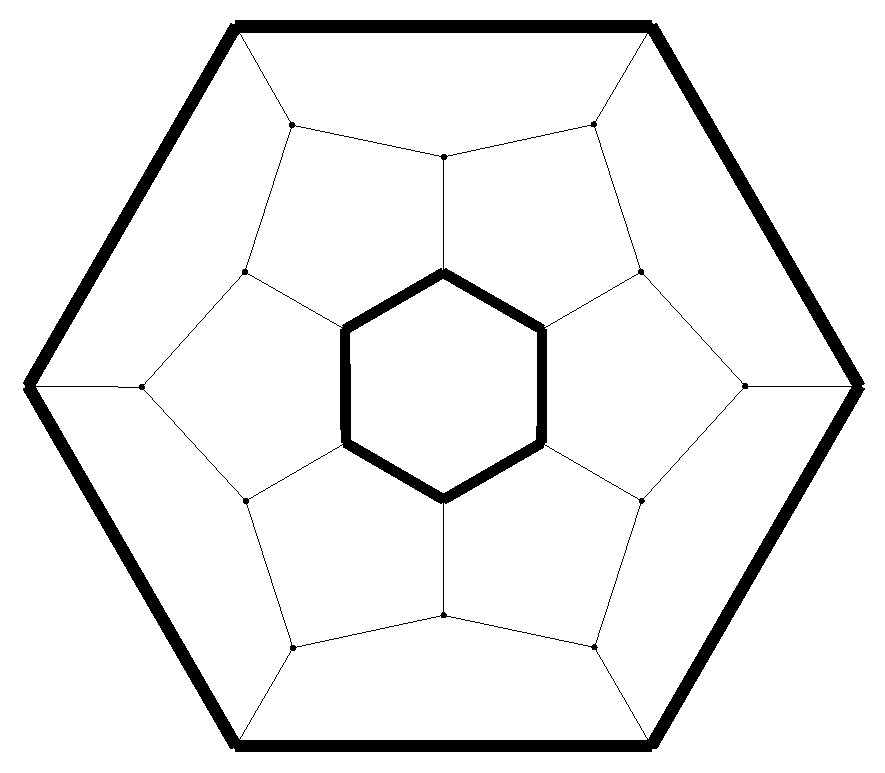
\epsfig{height=34mm, file=G1sec.eps}\par
\end{minipage}
\begin{minipage}{5.0cm}
\centering
\epsfig{height=34mm, file=G2sec.eps}\par
\end{minipage}
\begin{minipage}{5.0cm}
\centering
\epsfig{height=34mm, file=G3sec.eps}\par
\end{minipage}
\begin{minipage}{5.0cm}
\centering
\epsfig{height=34mm, file=G4sec.eps}\par
!!Add, perhaps, Barrel_q for q=3,4, but delete, if no place, for q=10, 9!!
\end{minipage}
\end{center}
}
\end{slide}
}


\begin{slide}{Euler formula}
\begin{itemize}
\item Let $G$ be a generalized $(p,3)$-polycycle with $t$ 
!!%boundaries.
holes.!!
\item $v_2$ and $v_3$ the number of vertices of degree $2$
!!%, 
and!! $3$ on $t$!! boundaries of all holes.
\item Let $x$ and $f_p$ be the number of interior vertices and $p$-gonal interior faces.
\end{itemize}
Then
!!%, 
one has:
\begin{equation*}
\left\lbrace\begin{array}{rcl}
pf_p-3x         &=& v_2+2v_3\\
f_p-\frac{x}{2} &=& (2-t)+\frac{v_3}{2}
\end{array}\right.
\end{equation*}


\end{slide}


\begin{slide}{}
\begin{center}
{\Huge 
\begin{tabular*}{7cm}{c}
\\[-0.5cm]
\textcolor{blue}{III. }\textcolor{red}{$pR_i$-maps}
\end{tabular*}
}
\end{center}
\end{slide}


\begin{slide}{$4R_0$-!! and $4R_1$-!!cases}
\begin{itemize}
\item $4R_0$-maps exist only for $q=7$ or $8$.
\begin{itemize}
\item For $q=7$, there is an infinity of spheres and tori.
\item For $q=8$, the only case is strictly face-regular $(4,8)$-torus 
$4R_0$, $8R_4$.
\end{itemize}
\item $4R_1$-maps exist only for $7\leq q\leq 10$
\begin{itemize}
\item For $q=7,8$, there is an infinity of spheres and tori.
\item For $q=9$,!! no sphere is known,!! but!! such!! tori!! exist:!!
\begin{center}
\begin{minipage}{5cm}
\centering
\resizebox{3.5cm}{!}{\includegraphics{FaceRegular/Torus49_4R1_2.eps}}\par
\end{minipage}
\end{center}
\item For $q=10$, only tori exist and they are $10R_4$.
\end{itemize}

\end{itemize}

\end{slide}




\begin{slide}{$4R_2$-!!case}
\begin{itemize}
\item $Prism_q$ is always $4R_2$. We consider maps different from $Prism_q$
\item $4$-gons are organized in triples.
\item One has $7\leq q\leq 16$ or $q=18$
\begin{itemize}
\item For $q=14$, $16$, $18$, they exist only on torus and are $qR_6$
\item Infinity of speheres is 
!!%proven 
found!!for $7\leq q\leq 10$ and $q=13$.
\item Uncertain 
!!%case is 
subcases!! are!! $q=11$, $13$ and $15$. Possible examples!! have
at least $92$, $116$ and $140$ vertices.
\end{itemize}
\end{itemize}

\end{slide}





\begin{slide}{$5R_1$-!! and $5R_2$-!!cases}
\begin{itemize}
\item $5R_1$ maps 
!!%exist only on torus and $q=7$ and 
are!! only!! $(5,7)$-tori!! and!! they!! are $7R_3$.
\item $5R_2$-maps exist only for $q=7$ 
!!%or 
and!! $8$.
\begin{itemize}
\item For $q=7$, there is an infinity of spheres (Hajduk \& Sotak) and tori.
\begin{center}
\begin{minipage}{5.0cm}
\centering
\resizebox{4.0cm}{!}{\includegraphics[bb=150 266 476 540, clip]{FaceRegular/Torus57_5R2_32.eps}}\par
\end{minipage}
\begin{minipage}{5cm}
\centering
\resizebox{4cm}{!}{\includegraphics{Boundary/Graph7_5_9-1newSec.eps}}\par
\end{minipage}
%\begin{minipage}{5.0cm}
%\centering
%\resizebox{4.0cm}{!}{\includegraphics[bb=150 266 476 540, clip]{FaceRegular/Torus57_5R2_68.eps}}\par
%\end{minipage}
\end{center}
\item For $q=8$, they exist only on torus!! and are also $8R_2$.
\end{itemize}

\end{itemize}

\end{slide}




\overlays{4}{
\begin{slide}{$5R_3$-!!case}
\onlySlide*{1}{
\begin{itemize}
\item The set of $5$-gons is decomposed 
!!%along 
into!! polycycles $E_1$!! and!! $E_2$:!!
\begin{center}
\begin{minipage}{3.7cm}
\centering
\epsfig{height=14mm, file=Polycycle/Fundamental22polycycle1.eps}\par
\end{minipage}
\begin{minipage}{3.7cm}
\centering
\epsfig{height=14mm, file=FaceRegular/Special7R5_Nr4.eps}\par
\end{minipage}
\end{center}
\item For $q=12$, they exist only on torus and are $12R_0$
\item For $q=11$, they exist only on torus and are $11R_1$
\begin{center}
\begin{minipage}{3.75cm}
\centering
\resizebox{3.3cm}{!}{\includegraphics[bb=150 266 476 540, clip]{FaceRegular/UniqueStrictly11R1_5R3.eps}}\par
\end{minipage}
\begin{minipage}{3.75cm}
\centering
\resizebox{3.3cm}{!}{\includegraphics[bb=150 266 476 540, clip]{FaceRegular/UniqueStrictly12R0_5R3.eps}}\par
\end{minipage}
\end{center}
\end{itemize}
}
\onlySlide*{2}{
\begin{itemize}
\item For $q=7$, they exist only on sphere and are:
\begin{center}
\begin{minipage}{5cm}
\centering
\resizebox{4.0cm}{!}{\includegraphics{FaceRegular/Graph57_5R3_7R1sec.eps}}\par
\end{minipage}
\begin{minipage}{5cm}
\centering
\resizebox{4.0cm}{!}{\includegraphics{FaceRegular/Missed57_5R3.ps}}\par
\end{minipage}
\end{center}



\end{itemize}
}
\onlySlide*{3}{
\begin{itemize}
\item For $q=9$, it exist only on sphere and is:
\begin{center}
\vspace{-2mm}
\begin{minipage}{11cm}
\centering
\resizebox{6.0cm}{!}{\includegraphics{FaceRegular/UNIQ_59_5R3sec.eps}}\par
%\textcolor{red}{Unique} $(5,9)$-spheres $5R_3$
\end{minipage}
\end{center}

\end{itemize}
}
\onlySlide*{4}{
\begin{itemize}
\item For $q=8$, an infinity of $(5,8)$-spheres is known. Two tori are known, one being $8R_4$, the other not.
\item For $q=10$, some spheres are known with $140$, $740$ and $7940$ vertices.
 Infinitness!! of spheres 
!!%is unknown 
and existence of tori, which are not 
$10R_2$,!! are!! undecided.!!
!!% is unclear.
\end{itemize}
}

\end{slide}
}

\begin{slide}{}
\begin{center}
{\Huge 
\begin{tabular*}{7cm}{c}
\\[-0.5cm]
\textcolor{blue}{III. }\textcolor{red}{$qR_0$-maps}
\end{tabular*}
}
\end{center}
\end{slide}




\begin{slide}{Frank-Kasper polyhedra}
\begin{itemize}
\item a \textcolor{red}{Frank-Kasper} polyhedron is a $(5,6)$-sphere,!! 
which is $6R_0$. Exactly $4$ cases exists!!.
\item A \textcolor{red}{space fullerene} is a face-to-face tiling of the Euclidean space $E^3$ by Frank-Kasper polyhedra. They appear in Crystallography of alloys and in bubble structures.
\end{itemize}

\begin{center}
\begin{minipage}{4.5cm}
\begin{minipage}{20mm}
\centering
\epsfxsize=17mm
\epsfbox{F1.ps}\par
\end{minipage}
\hfill\begin{minipage}{20mm}
\centering
\epsfxsize=20mm
\epsfbox{F2sec.eps}\par
\end{minipage}
\begin{minipage}{20mm}
\centering
\epsfxsize=20mm
\epsfbox{F3sec.eps}\par
\end{minipage}
\hfill\begin{minipage}{20mm}
\centering
\epsfxsize=20mm
\epsfbox{F4sec.eps}\par
\end{minipage}
\end{minipage}
\begin{minipage}{4.5cm}
\centering
\resizebox{4cm}{!}{\includegraphics[bb=176 30 420 267, clip]{fig14.eps}}\par
\end{minipage}
\end{center}

\end{slide}



\overlays{5}{
\begin{slide}{Polycycle decomposition}
\onlySlide*{1}{
\begin{itemize}
\item We consider $(5,q)$-spheres and tori, which are $qR_0$
\item \textcolor{red}
!!%{Thm.} 
The set of $5$-gonal faces of Frank-Kasper maps is 
decomposable!! along the frontiers into the following 
non-decomposable!! $(5,3)$-!!polycycles:
\begin{center}
\begin{minipage}{3.4cm}
\centering
\epsfig{height=18mm, file=Polycycle/Fundamental22polycycle1.eps}\par
$E_1$
\end{minipage}
\begin{minipage}{3.4cm}
\centering
\resizebox{3.0cm}{!}{\includegraphics{Polycycle/Fundamental22polycycle2.eps}}\par
$C_3$
\end{minipage}
\begin{minipage}{3.4cm}
\centering
\resizebox{3.0cm}{!}{\includegraphics{Polycycle/Fundamental22polycycle3.eps}}\par
$C_1$
\end{minipage}
\end{center}
\item The \textcolor{red}{major skeleton} $Maj(G)$ of a Frank-Kasper map 
is a $3$-valent map, whose vertex-set consists of polycycles $E_1$ 
and $C_3$.
!!not clear as now; perhaps, define edges?!!
\end{itemize}
}
\onlySlide*{2}{
\begin{center}
\begin{minipage}{8.4cm}
\centering
\resizebox{7.0cm}{!}{\includegraphics{Tripling514_14R0_1_C0.eps}}\par
A Frank-Kasper $(5,14)$-sphere
\end{minipage}
\end{center}
}
\onlySlide*{3}{
\begin{center}
\begin{minipage}{8.4cm}
\centering
\resizebox{7.0cm}{!}{\includegraphics{Tripling514_14R0_1_C1.eps}}\par
The polycycle decomposition
\end{minipage}
\end{center}
}
\onlySlide*{4}{
\begin{center}
\begin{minipage}{8.4cm}
\centering
\resizebox{7.0cm}{!}{\includegraphics{Tripling514_14R0_1_C2.eps}}\par
Their names
\end{minipage}
\end{center}
}
\onlySlide*{5}{
\begin{center}
\begin{minipage}{8.4cm}
\centering
\resizebox{7.0cm}{!}{\includegraphics{Tripling514_14R0_1_C3.eps}}\par
The major skeleton
\end{minipage}
\end{center}
}

\end{slide}
}


\begin{slide}{Results}
\begin{itemize}
\item For a Frank-Kasper $(5,q)$-map, the gonality of faces of $Maj(G)$ is at most $\lfloor \frac{q}{2}\rfloor$.
\item If $q<12$, then there is no $(5,q)$-tori $qR_0$ and there is a finite number of $(5,q)$-spheres $qR_0$.\\
For $q=12$:

\begin{minipage}{5.2cm}
\begin{itemize}
\item There is a unique $(5,12)$-torus $12R_0$
\item The $(5,12)$-spheres $12R_0$ are classified.
\end{itemize}
\vspace{0.7cm}
\end{minipage}
\begin{minipage}{5.2cm}
\centering
\resizebox{4.0cm}{!}{\includegraphics[bb=150 266 476 540, clip]{FaceRegular/UniqueStrictly12R0_5R3.eps}}\par
\end{minipage}
\item \textcolor{green}{Conjecture:!!} there is an infinity of 
$(5,q)$-spheres $qR_0$ for any $q>12$.
\end{itemize}
\end{slide}


\begin{slide}{}
\begin{center}
{\Huge 
\begin{tabular*}{7cm}{c}
\\[-0.5cm]
\textcolor{blue}{IV. }\textcolor{red}{$qR_1$-maps}
\end{tabular*}
}
\end{center}
\end{slide}



\begin{slide}{Euler formula}
If $P$ is a $(p,q)$-map, which is $qR_1$ ($q$-gons in isolated pairs), then:
\begin{equation*}
\left\lbrace\begin{array}{rl}
(6-p)x_3+(2(p-q)+(6-p)(q-1) )f_q=4p  &\mbox{~on~sphere},\\
(6-p)x_3+(2(p-q)+(6-p)(q-1) )f_q=0   &\mbox{~on~torus}.
\end{array}\right.
\end{equation*}
with $x_3$ being the number of vertices included in three $p$-gonal faces.

\begin{itemize}
\item For $(4,q)$-maps this yields finiteness on sphere and non-existence
on torus. 
\item For $(5,q)$-maps this implies finiteness on sphere for $q\leq 8$ and non-existence on torus
\end{itemize}

\end{slide}



\begin{slide}{Polycycle decomposition}
\vspace{-3mm}
\begin{itemize}
\item There is no $(4,q)$-sphere $qR_1$.
\item \textcolor{red}
!!%{Thm.} 
The non-decomposable!! $(5,3)$-polycycles,!! appearing in the 
decomposition are:
\begin{center}
\begin{minipage}{3.4cm}
\centering
\resizebox{2.0cm}{!}{\rotatebox{180}{\includegraphics{Polycycle/PolycycleD.eps}}}\par
\end{minipage}
\begin{minipage}{3.4cm}
\centering
\resizebox{2.5cm}{!}{\includegraphics{Polycycle/Fundamental22polycycle3.eps}}\par
\end{minipage}
\begin{minipage}{3.4cm}
\centering
\resizebox{2.0cm}{!}{\includegraphics{Polycycle/Elementary53_C2.eps}}\par
\end{minipage}
\begin{minipage}{3.4cm}
\centering
\resizebox{1.5cm}{!}{\includegraphics{Polycycle/Fundamental22polycycle2.eps}}\par
\end{minipage}
\begin{minipage}{3.4cm}
\centering
\epsfig{height=14mm, file=Polycycle/Fundamental22polycycle1.eps}\par
\end{minipage}
\end{center}
and the infinite serie $E_{2n}$ (see cases $n=1,2$ below):!!
\begin{center}
\begin{minipage}{4.7cm}
\centering
\epsfig{height=14mm, file=Polycycle/Elementary53_E2.eps}\par
!!%$E_2$
!!since you not fit as now!!
\end{minipage}
\begin{minipage}{4.7cm}
\centering
\epsfig{height=14mm, file=Polycycle/Elementary53_E4.eps}\par
!!%$E_4$
\end{minipage}
\end{center}

\end{itemize}
\end{slide}








\begin{slide}{$(5,9)$-maps $9R_1$}
\begin{itemize}
\item In the case $q=9$, Euler formula implies that the number of 
vertices,!! included in three $5$-gons,!! is bounded 
(\textcolor{red}{for!! sphere}) or zero (\textcolor{red}{for!! torus}).
\item All non-decomposable!! $(5,3)$-!!polycycles!! (except the single 
$5$-gon) contain such vertices. 
This implies \textcolor{red}{finiteness} on sphere and \textcolor{red}{non-existence} on torus.
\item While finiteness of $(5,q)$-spheres!! $qR_1$ is proved for $q=8$ and 
$q=9$, the actual work of enumeration is not finished.
\end{itemize}
\end{slide}




\begin{slide}{$(5,10)$-tori $10R_1$ and beyond}

\begin{itemize}
\item Using Euler formula and polycycle decomposition, 
!!%we proved 
one!! can!! see!! that the only appearing!! polycycles 
!!%appearing 
are:
\begin{center}
\begin{minipage}{3.4cm}
\centering
\resizebox{2.0cm}{!}{\rotatebox{180}{\includegraphics{Polycycle/PolycycleD.eps}}}\par
\end{minipage}
\begin{minipage}{3.4cm}
\centering
\epsfig{height=14mm, file=Polycycle/Fundamental22polycycle1.eps}\par
\end{minipage}
\end{center}
\item $(5.10)$-torus!!, which is $10R_1$,!! corresponds, in a one-to-one 
fashion, to a \textcolor{red}{perfect matching!!} of!! the!! $6$-regular 
triangulation!! of the torus,!! such that every vertex is contained in a 
triangle,!! whose opposite edges!! 
!!again, as in the beginning, any 2 edges of a triangle are opposite!!
belong to the perfect matching.
\item Existence of $(5,q)$-torus $qR_1$ for $q\geq 10$.
!!above line is not informative!!
\item \textcolor{green}{Conjecture:!!} there!! exists!! an infinity of 
$(5,q)$-spheres!! $qR_1$ for any!! $q\geq 10$.
\end{itemize}

\end{slide}







\begin{slide}{}
\begin{center}
{\Huge 
\begin{tabular*}{8cm}{c}
\\[-0.5cm]
\textcolor{blue}{V. }\textcolor{red}{$qR_2$-maps}\\
\end{tabular*}
}
\end{center}
\end{slide}









\begin{slide}{Euler formula}
\begin{itemize}
\item One has the Euler formula
\begin{equation*}
(4-(4-p)(4-q))f_q+(6-p)(\textcolor{red}{x_1}+\textcolor{red}{x_2})=4p, \mbox{,~{\em where}}
\end{equation*}
\begin{itemize}
\item \textcolor{red}{$x_1$} is the number of vertices incident to $3$ $p$-gonal faces and
\item \textcolor{red}{$x_2$} the number of vertices incident to $3$ $q$-gonal faces.
\end{itemize}
\item \textcolor{red}{finiteness} for $(4,q)$, $(5,6)$, $(5,7)$ but we have \textcolor{red}{infinity} for $(6,5)$ and, possibly, for $(5,q)$, $q\geq 8$.
!!as now, not clear, is it for one ring on sphere or more general!!

\end{itemize}

\end{slide}










\begin{slide}{All!! $(4,q)$-maps $qR_2$}
\begin{itemize}
\item two possibilities (for $q=8,6$)!!:

\begin{center}
\begin{minipage}{3cm}
\centering
\resizebox{2.4cm}{!}{\includegraphics{Boundary/M2_4_8.ps}}\par
\end{minipage}
\begin{minipage}{3cm}
\centering
\resizebox{2.4cm}{!}{\includegraphics{Boundary/M3_4_6.ps}}\par
\end{minipage}
\end{center}
\item \textcolor{red}{and} 
!!%an 
the!! infinite series!!\\[1mm]
\begin{center}
\begin{minipage}{2.6cm}
\centering
\resizebox{2.4cm}{!}{\includegraphics{Boundary/InfiniteStep5sec.eps}}\par
\end{minipage}
\begin{minipage}{2.6cm}
\centering
\resizebox{2.4cm}{!}{\includegraphics{Boundary/Infinite6-1sec.eps}}\par
\end{minipage}
\begin{minipage}{2.6cm}
\centering
\resizebox{2.6cm}{!}{\includegraphics{Boundary/Infinite7-1this.eps}}\par
\end{minipage}
\begin{minipage}{2.6cm}
\centering
\resizebox{2.4cm}{!}{\includegraphics{Boundary/Infinite8-1sec.eps}}\par
\end{minipage}
\end{center}
\end{itemize}

\end{slide}




\begin{slide}{$(5,q)$-maps $qR_2$}
\begin{itemize}
\item For $q=6$, $7$ the list of spheres is known. No tori!! in 
!!%that 
those!! cases.
\item For $q\geq 8$, then there is an infinity of maps.
!!In above and below lines precise maps: spheres/tori!!
\item a $(5,8)$-map is $8R_2$ if and only if it is $5R_2$
\item For any!! $q\geq 8$, there is $(5,q)$-torus!! $qR_2$.

\end{itemize}
\end{slide}
















\begin{slide}{}
\begin{center}
{\Huge 
\begin{tabular*}{7cm}{c}
\\[-0.5cm]
\textcolor{blue}{III. }\textcolor{red}{$qR_3$-maps}
\end{tabular*}
}
\end{center}
\end{slide}






\begin{slide}{Classification for $(4,q)$-case}
\begin{itemize}
\item The $(4,3)$-polycycles, appearing in the decomposition, are:
\begin{center}
\epsfig{figure=Boundary/DiscreteCase4gonalPatchNOB.eps,width=6cm}
\end{center}
\begin{center}
\epsfig{figure=Boundary/InfiniteSequenceNOB.eps,width=8cm}
\end{center}

\item Consider the map whose faces are $q$-gonal faces of a $(4,q)$-sphere $qR_3$.
\begin{itemize}
\item It is a $3$-valent map
\item Its faces are $2$-, $3$- or $4$-gons.
\item It has at most $8$ vertices.
\end{itemize}
!!now you not fit; perhaps, put above 3 items in common line!!
\end{itemize}
\end{slide}


\overlays{3}{
\begin{slide}{}
\onlySlide*{1}{
\begin{itemize}
\item \epsfig{figure=Bundle.eps,width=2cm} yields 
\epsfig{figure=FaceRegular/Missed12Rsec.eps, width=2cm}
\item \epsfig{figure=Tetrahedron.ps,width=2cm} yields 
\epsfig{figure=FaceRegular/FaceRegular/35sec.eps, width=2cm}
\item \epsfig{figure=Dihedre.eps,width=2cm} yields 
\epsfig{figure=FaceRegular/WeakAzul49_9R3_2thi.eps, width=2cm} (one infinite series)
\end{itemize}
}
\onlySlide*{2}{
\begin{itemize}
\item \epsfig{figure=Prism3_naked.eps,width=2cm} yields
\begin{center}
\epsfig{figure=FaceRegular/WeakAzul49_9R3_3sec.eps, width=4cm}
and 
\epsfig{figure=FaceRegular/WeakAzul49_9R3_4sec.eps, width=4cm}
\end{center}
\begin{center}
(two infinite series)
\end{center}
\end{itemize}
}
\onlySlide*{3}{
\begin{itemize}
\item \epsfig{figure=Cube.eps,width=1.5cm} yields
\begin{center}
\epsfig{figure=FaceRegular/WeakAzul49_9R3_6sec.eps, width=4cm}
\epsfig{figure=FaceRegular/WeakAzul49_9R3_5sec.eps, width=4cm}
\end{center}
(multiple 
!!unclear above: infinity or many of them?!!
infinite series)
\end{itemize}
}
\end{slide}
}


\begin{slide}{$(5,q)$-maps $qR_3$}
\begin{itemize}
\item A $(5,7)$-torus, which is $7R_3$, is also $5R_1$.
\item A $(5,7)$-sphere, which is $7R_3$, has $x_0+x_3=20$ with $x_i$ being the number of vertices contained in $i$ $5$-gonal faces.
\item For all $q\geq 7$, $(5,q)$-tori, $qR_3$ are known:
\begin{center}
\begin{minipage}{3.5cm}
\centering
\resizebox{3.3cm}{!}{\includegraphics[bb=150 266 476 540, clip]{FaceRegular/Torus58_8R3_1.eps}}\par
\end{minipage}
\begin{minipage}{3.5cm}
\centering
\resizebox{3.3cm}{!}{\includegraphics[bb=150 266 476 540, clip]{FaceRegular/Torus59_9R3_1.eps}}\par
\end{minipage}
\begin{minipage}{3.5cm}
\centering
\resizebox{3.3cm}{!}{\includegraphics[bb=150 266 476 540, clip]{FaceRegular/Torus510_10R3_1.eps}}\par
\end{minipage}
\end{center}
\item \textcolor{green}{Conj.} For any $q\geq 7$ there is an infinity of $(5,q)$-spheres.
\end{itemize}

\end{slide}





\begin{slide}{}
\begin{center}
{\Huge 
\begin{tabular*}{7cm}{c}
\\[-0.5cm]
\textcolor{blue}{III. }\textcolor{red}{$qR_4$-maps}
\end{tabular*}
}
\end{center}
\end{slide}





\overlays{3}{
\begin{slide}{Classification of $(4,8)$-spheres $8R_4$}
\onlySlide*{1}{
\begin{itemize}
\item For $(4,8)$-maps, which are $8R_4$, one has
\begin{equation*}
\begin{array}{rcl}
x_0+x_3&=&8(1-g)\\
e_{4_4}&=&12(1-g)
\end{array}
\end{equation*}
with $g$ being the genus.
\item There exists an unique $(4,8)$-torus $8R_4$:
\begin{center}
\begin{minipage}{3.5cm}
\centering
\resizebox{2.3cm}{!}{\includegraphics[bb=150 266 476 540, clip]{FaceRegular/UniqueTorus48_8R4.eps}}\par
\end{minipage}
\end{center}
\item We use an exhaustive enumeration method.

%Reason for expecting success:
%\begin{itemize}
%\item two conservation laws that allow to destroy a lot of unfinished graphs.
%\item only one structure opf torus, which means that the large scale structure of the sphere should be very uniform with a few wrinkles.
%\end{itemize}
\end{itemize}
}
\onlySlide*{2}{
\begin{center}
\begin{minipage}{5cm}
\centering
\resizebox{4.0cm}{!}{\includegraphics{FaceRegular/WeakAzul48_8R4_14sec.eps}}\par
\end{minipage}
%\begin{minipage}{5cm}
%\centering
%\resizebox{4.0cm}{!}{\includegraphics{FaceRegular/WP3_5.ps}}\par
%\end{minipage}
%\begin{minipage}{5cm}
%\centering
%\resizebox{4.0cm}{!}{\includegraphics{FaceRegular/WP2_16sec.eps}}\par
%\end{minipage}
\begin{minipage}{5cm}
\centering
\resizebox{4.0cm}{!}{\includegraphics{FaceRegular/DRA_200_Ohsec.eps}}\par
\end{minipage}
\end{center}
\begin{center}
Some sporadic spheres among $78$ sporadic spheres.!!
\end{center}
}
\onlySlide*{3}{
\begin{center}
\begin{minipage}{5cm}
\centering
\resizebox{3.0cm}{!}{\includegraphics{FaceRegular/WeakAzul48_8R4_1.ps}}\par
\end{minipage}
\begin{minipage}{5cm}
\centering
\resizebox{3.0cm}{!}{\includegraphics{FaceRegular/WeakAzul48_8R4_2sec.eps}}\par
\end{minipage}
\begin{minipage}{5cm}
\centering
\resizebox{3.0cm}{!}{\includegraphics{FaceRegular/WeakAzul48_8R4_3thi.eps}}\par
\end{minipage}
\begin{minipage}{5cm}
\centering
\resizebox{3.0cm}{!}{\includegraphics{FaceRegular/WeakAzul48_8R4_6sec.eps}}\par
\end{minipage}
\end{center}
\begin{center}
One infinite series amongst!! $13$ infinite series.!!
\end{center}


}


\end{slide}
}









\begin{slide}{}
\begin{center}
{\Huge 
\begin{tabular*}{7cm}{c}
\\[-0.5cm]
\textcolor{blue}{III. }\textcolor{red}{$qR_5$-maps}
\end{tabular*}
}
\end{center}
\end{slide}


\begin{slide}{$(4,q)$-case}
\begin{itemize}
\item $(4,q)$-tori!!, which are $qR_5$,!! are known for any $q\geq 7$.
\item For $q=7$, they are $4R_0$.
\item $(4,7)$-spheres $7R_5$ satisfy!! to $e_{4-4}=12$. Is there an 
infinity of such spheres?
\begin{center}
\begin{minipage}{3.5cm}
\centering
\resizebox{3.3cm}{!}{\includegraphics{FaceRegular/Example47_7R5thi.eps}}\par
\end{minipage}
\end{center}

\end{itemize}
\end{slide}




\begin{slide}{$(5,q)$-case}
\vspace{-3mm}
\begin{itemize}
\item The smallest $(5,q)$-spheres 
!!%which are 
$qR_5$ 
!!%are 
for $q=7$, $8$, $9$ are!!:
\begin{center}
\begin{minipage}{4.0cm}
\centering
\resizebox{3.8cm}{!}{\includegraphics{azulenoid/f-05-07a-schlegel.ps}}\par
\end{minipage}
\hspace{2.0cm}
\begin{minipage}{4.0cm}
\centering
\resizebox{3.8cm}{!}{\includegraphics{FaceRegular/Example58_8R5_2sec.eps}}\par
\end{minipage}
\end{center}
\vspace{-17mm}
\begin{center}
\begin{minipage}{4.0cm}
\centering
\resizebox{3.8cm}{!}{\includegraphics{FaceRegular/WeakAzul59_9R5_1sec.eps}}\par
\end{minipage}
\end{center}

\end{itemize}
\end{slide}





\end{document}

